%---------------------------------------------------------------------
% Course 	: Introduction To web sciences
% Professor : Dr.Nelson
% Name   	: Msnoj Chandra Kompalli
% Assignment: 8
%---------------------------------------------------------------------
\documentclass[12pt]{article}
%--------------------------------------------------------------------
% packages required
%--------------------------------------------------------------------
\usepackage{graphicx}
\usepackage{listings}
\usepackage{hyperref}
\usepackage{caption}
\usepackage{color}
\usepackage{pdfpages}
\graphicspath{ {images/} }
%--------------------------------------------------------------------
% Start Margins
%--------------------------------------------------------------------
\addtolength{\oddsidemargin}{-.875in}
\addtolength{\evensidemargin}{-.875in}
\addtolength{\textwidth}{1.75in}
\addtolength{\topmargin}{-.885in}
\addtolength{\textheight}{1.95in}
%-------------------------------------------------------------------
% End Margins
%--------------------------------------------------------------------
\definecolor{codegreen}{rgb}{0,0.6,0}
\definecolor{codegray}{rgb}{0.5,0.5,0.5}
\definecolor{codepurple}{rgb}{0.58,0,0.82}
\definecolor{backcolour}{rgb}{0.95,0.95,0.92}
 
\lstdefinestyle{mystyle}{
    backgroundcolor=\color{backcolour},   
    commentstyle=\color{codegreen},
    keywordstyle=\color{magenta},
    numberstyle=\tiny\color{codegray},
    stringstyle=\color{codepurple},
    basicstyle=\footnotesize,
    breakatwhitespace=false,         
    breaklines=true,                 
    captionpos=b,                    
    keepspaces=true,                 
    numbers=left,                    
    numbersep=5pt,                  
    showspaces=false,                
    showstringspaces=false,
    showtabs=false,                  
    tabsize=2
}
 
\lstset{style=mystyle}

\begin{document}

\begin{titlepage}
\title{INTRODUCTION TO WEB SCIENCES:\\*Assignment 8}
\author{Manoj Chandra Kompalli}
\date{7 April 2016}
\maketitle
\end{titlepage}

\tableofcontents
\newpage

\section{Question 1:  }


\subsection{Approach}
\begin{itemize}
\item I have extracted the 98 URIs initially and appended the required string 
\item I made sure there are no duplicates
\item I have added the given 2 URIs in the question to make it 100
\item I used feed parser to parse all the randomly generated URIs 
\item To get the most popular words I kept track of occurrence of each word in the blog
\item I sorted all the words based on how many times they occurred and selected the top 500 words.
\item Then I calculated the occurrence of every word in the respective blog
\item The resulting matrix contains 501 columns and 101 rows
\end{itemize}



 \newpage

\subsection{Code Listing}
\subsubsection{getBlogs.py to generate 100 URIs}
\lstinputlisting[breaklines=True,language=Python]{../../q1/getBlogs.py}
\newpage
\subsubsection{countPages.py to find the number of pages in each blog }
\lstinputlisting[breaklines=True,language=Python]{../../q1/countPages.py}
\newpage
\subsubsection{matrixcreate.py to create a blog term matrix }
\lstinputlisting[breaklines=True,language=Python]{../../q1/matrixcreate.py}
\newpage


\subsection{Blog term matrix shown in Excel }
\begin{figure}[ht]
\includegraphics[scale=0.7]{../../q1/output.png}
\centering
\caption{JSON array containing the follower data}
\label{fig:JSON array containing the follower data}
\end{figure}





\newpage
\section{Question 2: }

\subsection{Approach}
\begin{itemize}
\item I have used the clusters.py program mentioned in the presentation to produce the required dendogram
\item Printclust prints the dendogram 
\item drawdendogram saves it in JPEG format
\item There are numerous blogs similar to F-measure. The top one is the power of independent study
\item The blog similar to web science and Digital libraries Research group is Ideal copy
\end{itemize}

\subsection{Code Listing}
\subsubsection{dgram.py}
\lstinputlisting[breaklines=True,language=Python]{../../q2/dgram.py}
\newpage

\subsection{Output}

\subsubsection{JPEG Dendogram}
\begin{figure}[ht]
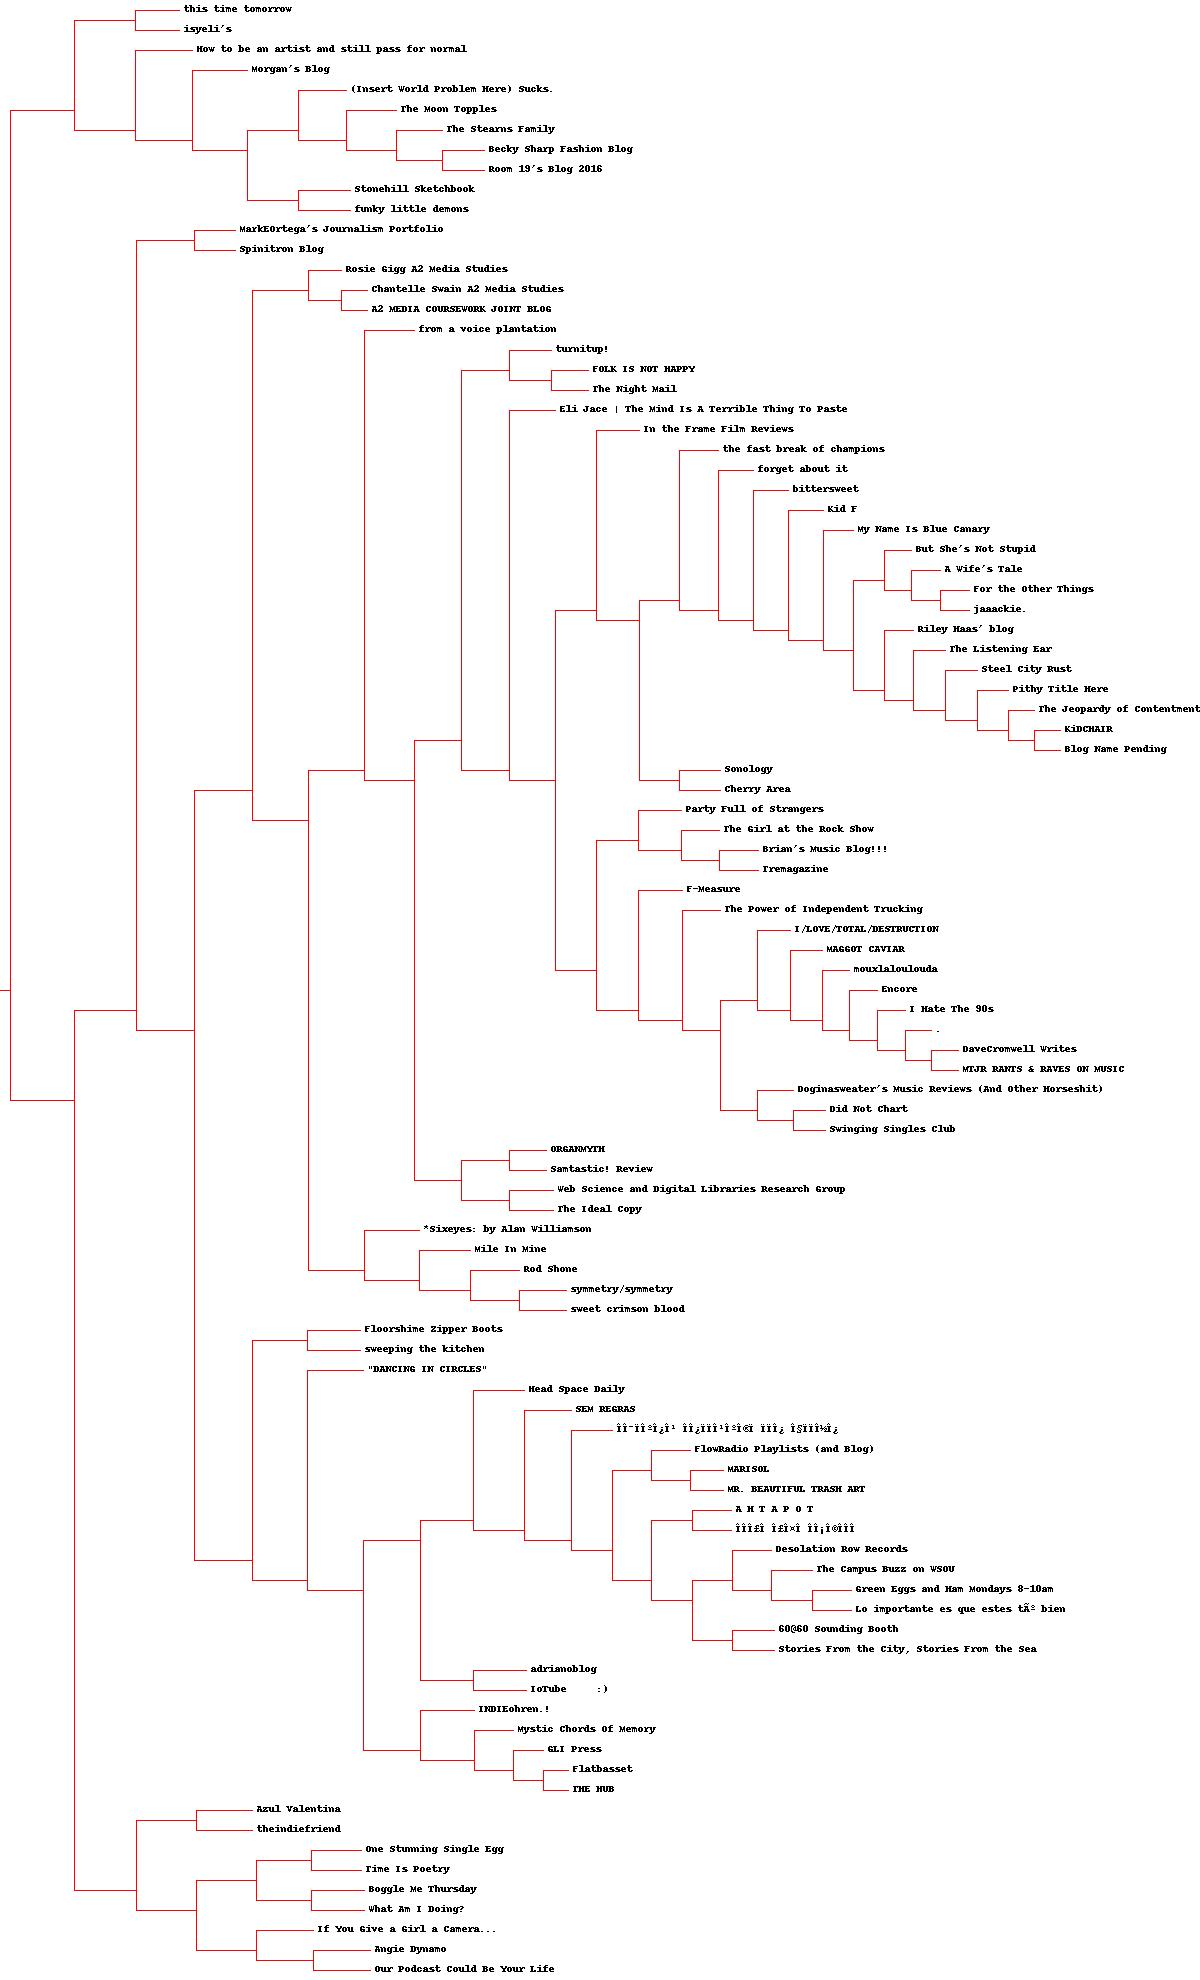
\includegraphics[scale=0.2]{../../q2/dendogram.jpg}
\centering
\caption{Initial graph split into 4 groups}
\label{Initial graph split into 4 groups}
\end{figure}
\newpage
\subsubsection{ASCII dendogram}
\lstinputlisting[breaklines=True,language=Python]{../../q2/ascii.txt}
\newpage



\section{Question 3: }
\subsection{Approach}
\begin{itemize}
\item Below code performs blog clustering based on clusters.py program using the method kcluster
\item The program prints the iterations involved for each values of k (5,10,20).
\item The program also print the values in each centroid for respective k values
\end{itemize}


\subsection{Code Listing}
\subsubsection{convert.py}
\lstinputlisting[breaklines=True,language=Python]{../../q3/kmean.py}
\newpage


\subsection{Output}
\subsubsection{Centroid Values and Iterations}
\begin{figure}[ht]
\includegraphics[scale=0.6]{../../q3/output.png}
\centering
\caption{Centroid Values and Iterations}
\label{Centroid Values and Iterations}
\end{figure}



\newpage
\section{Question 4: }
\subsection{Approach}
\begin{itemize}
\item Blog space is generated by the multi dimensional scaling using the code mds.py.
\item  Again we make use of clusters.py for the scaledown method. 
\item The output shows a graph which is circular unlike the previous question
\end{itemize}
\subsection{Code Listing}
\lstinputlisting[breaklines=True,language=Python]{../../q4/mds.py}
\newpage

\subsection{Output}
\subsubsection{JPEG of blogs using MPS}
\begin{figure}[ht]
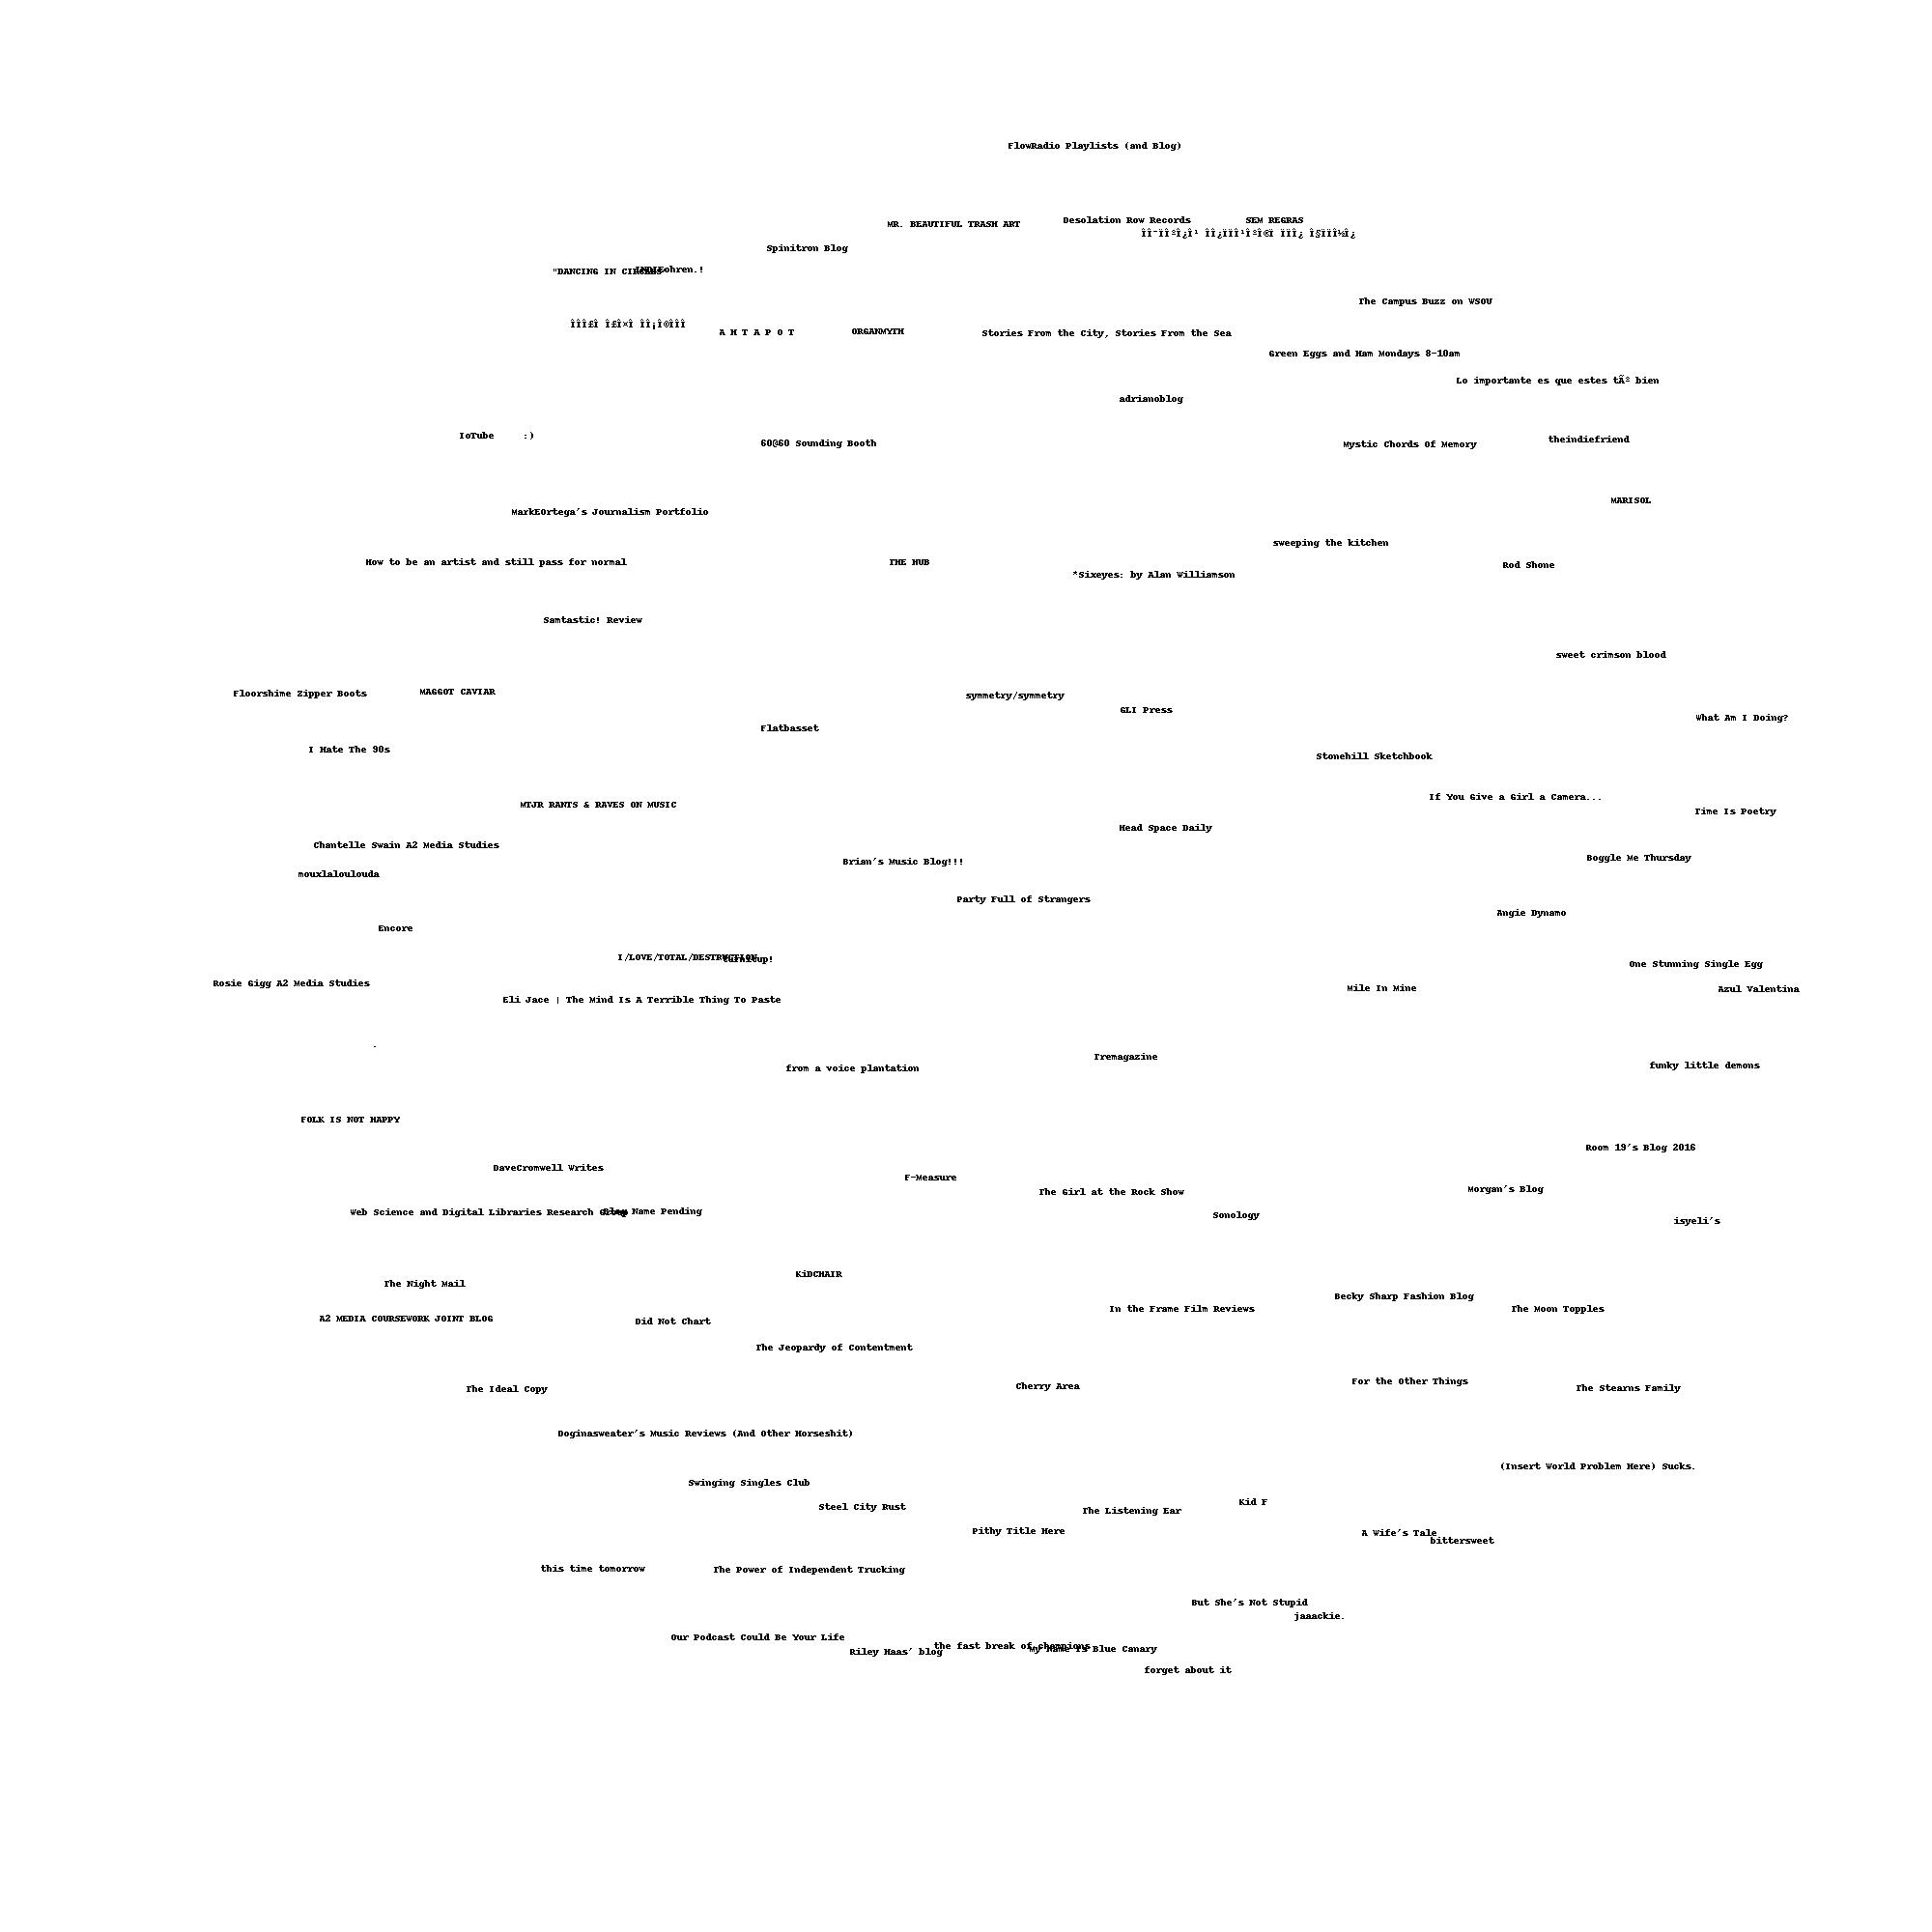
\includegraphics[scale=0.2]{../../q4/draw2d.jpg}
\centering
\caption{JPEG of blogs using MPS}
\label{JPEG of blogs using MPS}
\end{figure}
\newpage
\section{Question 5: }
\subsection{Approach}
\begin{itemize}
\item I wrote almost the same code except for the few lines which calculate the tfidf values
\item Here I have ordered the matrix based on tfidf values of the respective words.
\item I have extracted the words with high tfidf  values 
\item I generated  dendogram again just like how I did before.
\item From the current dendogram F-Measure is similar to the blog Desolation Row Records
\item WebScience and Digital Libraries Research Search group is similar to Maggot Caviar and blog I love total destruction 
\item We can observe that the hierarchy of the blogs has changed. Somehow, F-Measure now has a lot less similar blogs 
\end{itemize}

\subsection{Code Listing}
\lstinputlisting[breaklines=True,language=Python]{../../q5/tfidfmatrix.py}
\newpage
\subsection{Output}
\subsubsection{Output Blog term matrix with tfidf values}
\begin{figure}[ht]
\includegraphics[scale=0.7]{../../q5/output.png}
\centering
\caption{Output Blog term matrix with tfidf values}
\label{Output Blog term matrix with tfidf values}
\end{figure}
\newpage
\subsubsection{Output JPEG}
\begin{figure}[ht]
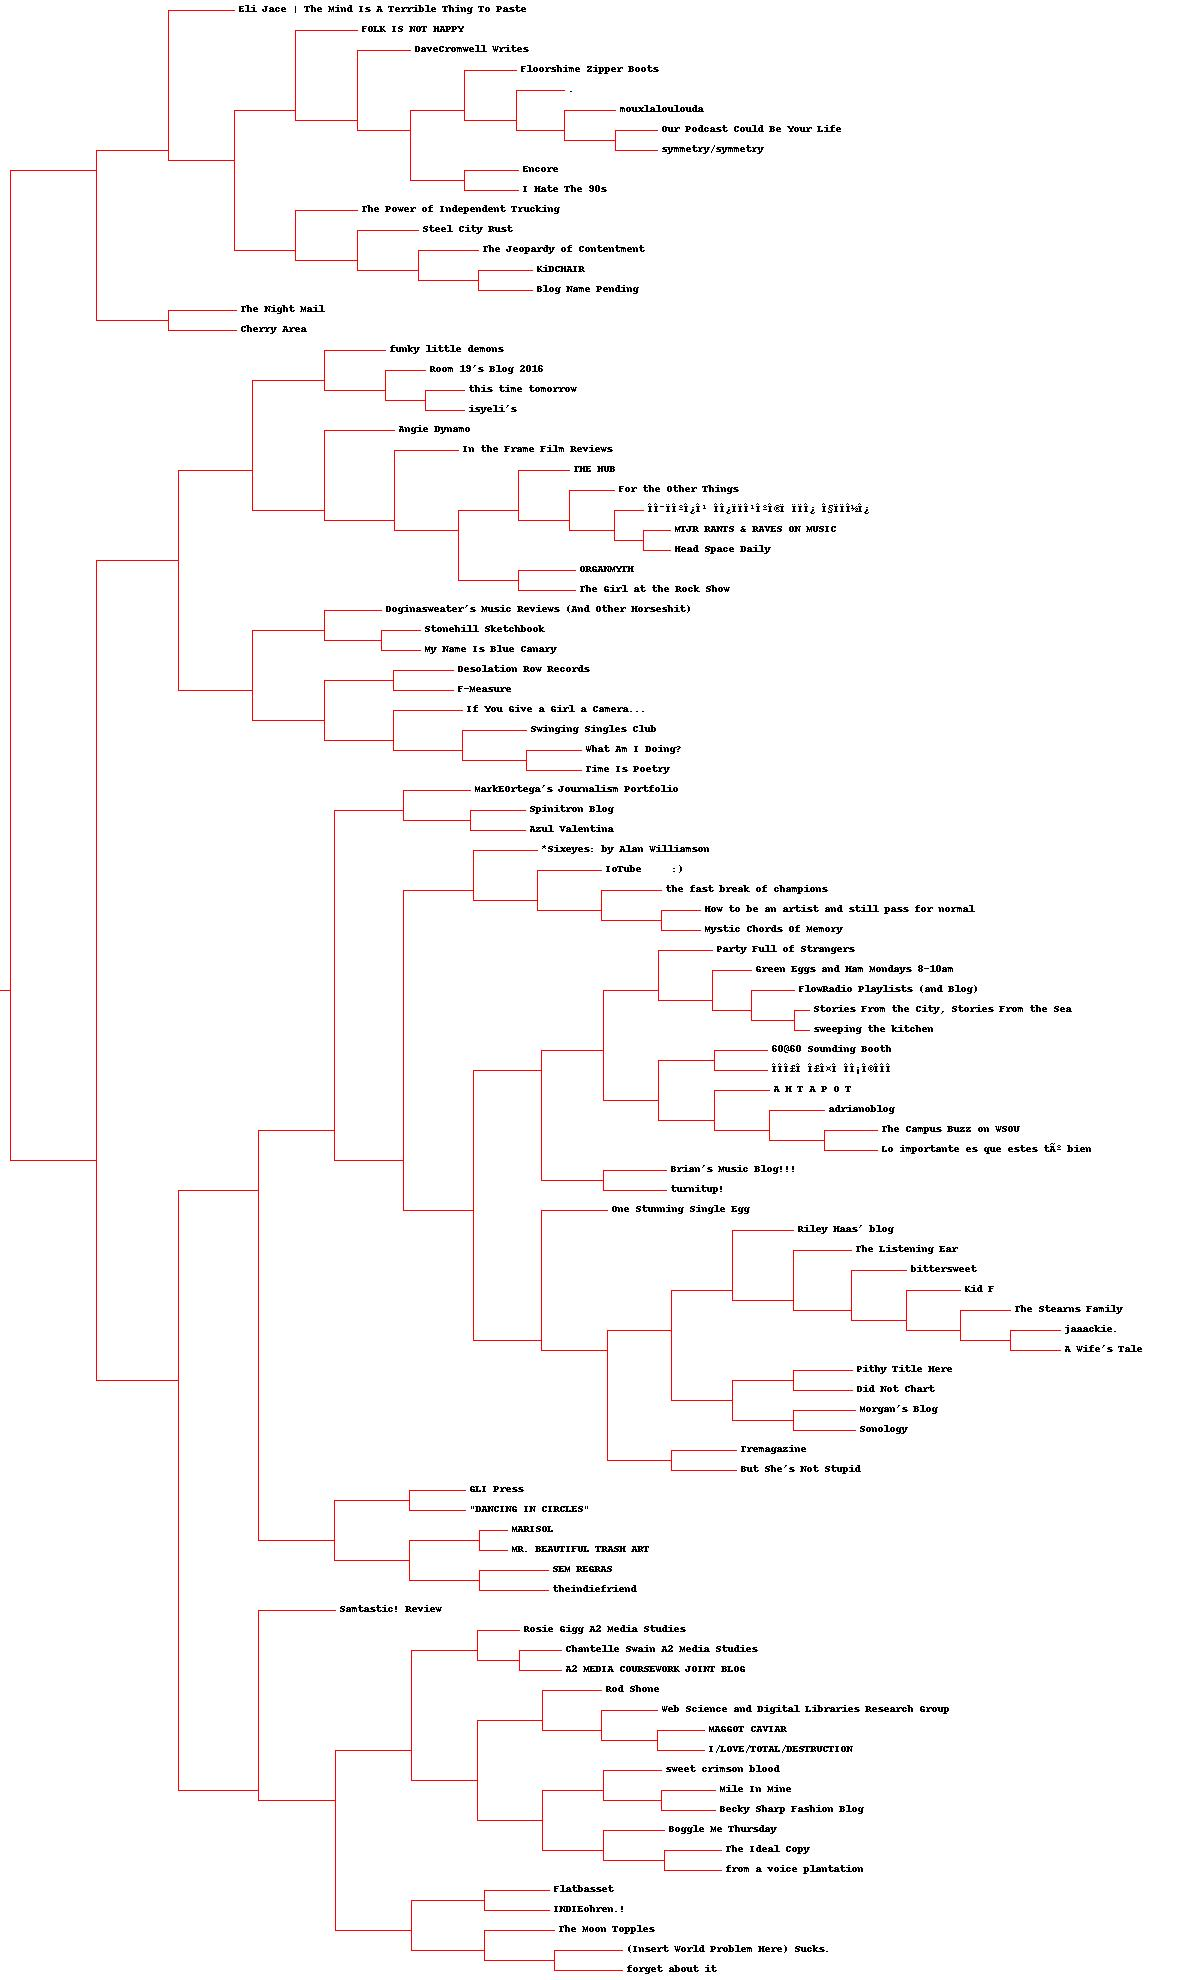
\includegraphics[scale=0.2]{../../q5/dendogram.jpg}
\centering
\caption{Output generated by mds.py}
\label{Output generated by mds.py}
\end{figure}
\newpage
\bibliographystyle{plain}
\bibliography{references}
\cite{*}
\end{document}